\chapter{Maori Culture - Digital library}

\section{Project analysis}
\subsection{Maori Culture}
Maori culture refers to the culture of the Maori people, the indigenous people of New Zealand. The Maori are the indigenous people of New Zealand. They have a rich history and cultural tradition that includes a unique language, art, music, dance, traditional medicine, architecture and food.

\begin{figure}[htbp]
  \centerline{\includegraphics[width=500pt]{images/MaoriCulture.jpg}}
\end{figure}

In order to promote Maori culture around the world, our project as a digital library platform will focus on presenting Maori culture based on the Maori language and supplemented by English.

\subsection{Project Objects}
The content of our project - Maori Cultural Digital Library is very rich and diverse. It mainly includes the following aspects, some of which can be made into electronic materials. Include: Maori language and culture Materials, Maori Arts and Crafts,Maori History and Cultural Geography.

\subsection{Project Content}
The content format of digital library is mainly based on the following formats:
E-Books, Video and audio files, Image and text documents, Interactive Applications.

\begin{figure}[htbp]
  \centerline{
\includegraphics[width=500pt]{images/digitallibrary.jpg}}
\end{figure}

\subsection{Project Direction}
Our project can be made into a digital library of Maori culture, which aims to collect, preserve, display and disseminate the Maori cultural heritage online platform.

The Maori Cultural Library initially provides curriculum education to young people (13-18 years old). It integrates Maori language lessons into textbooks and provides a Maori language learning environment for teenagers.

Digital Collection of Maori Cultural Heritage: The Maori Cultural Digital Library collects important Maori heritage such as traditional culture, history, art and language through digital technology, forming a digital cultural database, so that more people can easily access and understand Maori culture.

Promoting the inheritance and development of Maori culture: The Digital Library of Maori Culture is not only a platform for the collection and preservation of cultural heritage, but also an important tool for promoting the inheritance and development of Maori culture. Through digital display and dissemination, more people can learn and understand Maori culture, and help Maori themselves better protect and pass on their own culture.

Providing education and research resources: The Digital Library of Maori Culture is not only a showcase, it also provides a wealth of education and research resources, so that students, teachers and researchers can understand and study Maori culture more deeply, and promote the development of Maori cultural research.

Collaboration with other cultural digital libraries: Maori cultural digital libraries can collaborate with other cultural digital libraries to share cultural resources and experiences and enhance cultural exchange and understanding. In this way, more people can know about Maori culture, and at the same time, Maori can better understand and respect other cultures.

Protecting and inheriting the sustainability of Maori Culture: The Maori Cultural Digital Library is an important tool for protecting and inheriting Maori culture, which needs to be constantly updated and improved to ensure the sustainability of Maori cultural heritage. At the same time, it is also necessary to actively participate in community cultural activities to promote the development and inheritance of Maori culture.
 
\section{Digital Library}
Digital library refers to the library that uses digital technology to store, organize, retrieve, transmit, utilize and protect document resources. Different from traditional physical libraries, digital libraries are mainly dominated by literature resources in electronic form, which can be retrieved and accessed through computer networks. Digital library is the product of the information age. It uses the digital way to manage the document resources, which makes it more convenient for people to obtain and use the information resources, and also provides a broader space for academic research and education.

Digital library is of great significance to academic research and education. It provides more extensive and deeper information resources for education and research, and provides a more convenient and efficient learning, research and teaching platform for scholars, researchers and students. At the same time, digital library also provides a wider range of cultural and knowledge resources for the society, and promotes cultural exchange and knowledge innovation.

\begin{figure}[htbp]
  \centerline{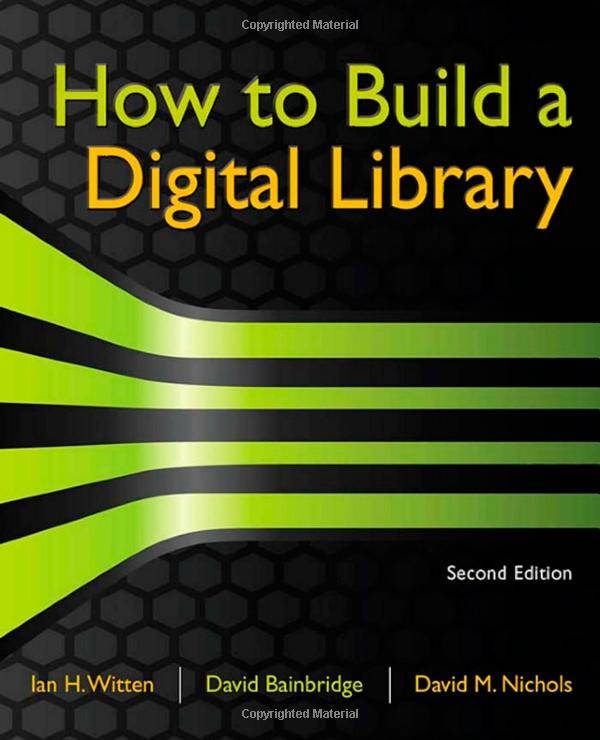
\includegraphics[width=500pt]{images/HowtoBuildDigitalLibrary.jpg}}
\end{figure}

\subsection{Main Features}
The main features of a digital library include:
Electronic resources, Resource sharing, Search function, Knowledge management, Globally, etc.

\subsection{Content}
In general, digital library includes literature resources, metadata, search tools, digital library systems, services and support, and rights management. These contents together constitute the basic elements of digital library, providing users with convenient, fast and efficient information resources services.
Literature resources,Metadata,Search tools, Digital library system, Services and Support, Copyright Management.

\subsection{Usage}
In order to give full play to the role of digital library, enterprises should ensure the effective protection of information retrieval, knowledge management, training and education after the establishment of digital library system. Enterprises also need to be equipped with special digital library administrators, responsible for the maintenance and update of digital library, to ensure that the resources and functions of digital library always keep the latest, the most comprehensive, the most valuable.

\subsection{Cost}
In general, most of the cost of digital library lies in the establishment and maintenance. However, the advantage of digital library is that it can greatly save the storage space and maintenance cost of traditional library, and digital library can provide richer and more convenient resources and services to bring better experience for users.
 
